\documentclass[letterpaper, 11pt]{article}

% Standard packages
\usepackage{amsmath, amsthm, latexsym, amssymb, graphicx, color, mathtools, geometry}

% Simplifies margin settings
\usepackage{geometry}
\geometry{margin=1in,headsep=.25in}

% Puts list item indicators in bold; makes flush with previous margin
\renewcommand\labelenumi{\bf\theenumi.}
\renewcommand\labelenumii{\bf\theenumii.}
\setlength\leftmargini{1.4em}
\setlength\leftmarginii{1.4em}

% Flexibility for headers and footers
\usepackage{fancyhdr}
\usepackage{datetime2}
\usepackage{float}

\pagestyle{fancyplain}
\fancyhf{} %clear all header and footer fields
\cfoot{\bf \small Page \thepage}
\headsep 0.2in
\thispagestyle{empty}

\usepackage[pdftex]{hyperref}
\hypersetup{
    unicode=false,          % non-Latin characters in Acrobat's bookmarks
    pdftoolbar=true,        % show Acrobat's toolbar?
    pdfmenubar=true,        % show Acrobat's menu?
    pdffitwindow=true,      % page fit to window when opened
    pdftitle={My title},    % title
    pdfauthor={Author},     % author
    pdfsubject={Subject},   % subject of the document
    pdfnewwindow=true,      % links in new window
    pdfkeywords={keywords}, % list of keywords
    colorlinks=true,        % false: boxed links; true: colored links
    linkcolor=black,        % color of internal links
    citecolor=green,        % color of links to bibliography
    filecolor=magenta,      % color of file links
    urlcolor=blue           % color of external links
}

\renewcommand{\headrulewidth}{0pt}

\parindent 0in
\parskip 12pt

\begin{document}

\title{Homework Template}

\begin{center}
    {
        \large
        \bf
        CS-E4850 Computer Vision\\
        Exercise Round \#9\\
        Submitted by Chen\ Xu, ID 000000\\
        \today
    }
\end{center}
\bigskip
\textbf{Exercise 1. Neural networks and backpropagation.}

\begin{figure}[H]
    \centering
    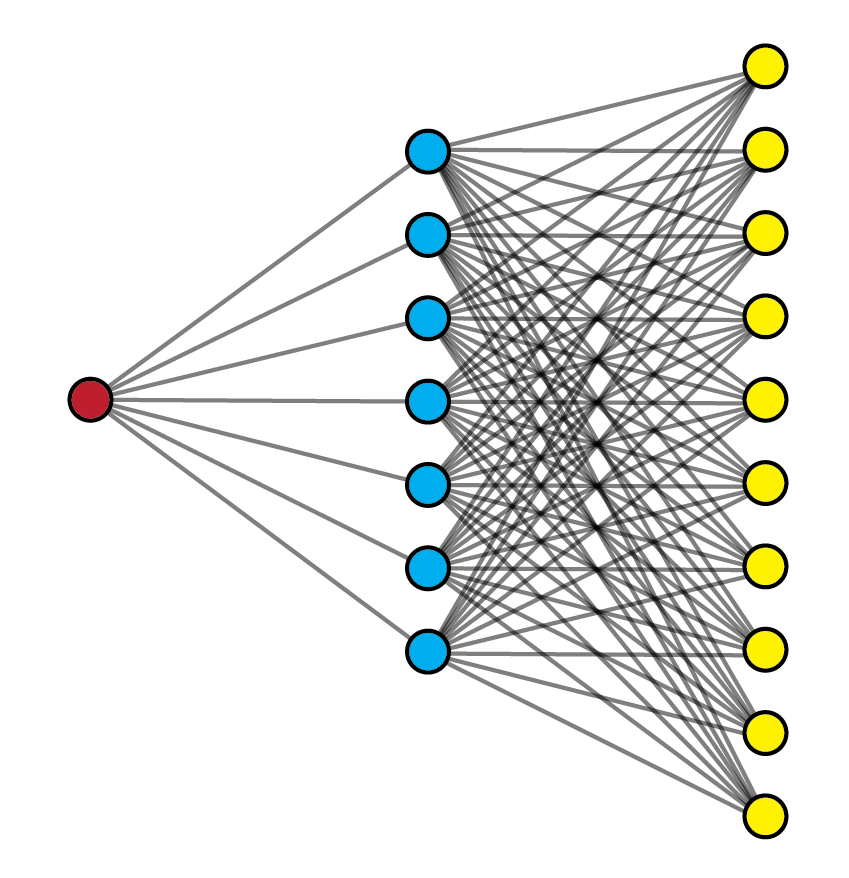
\includegraphics{ex9NN-01.png}
    \caption{Schematics of a neural network}
    \label{fig:schematics}
\end{figure}

1)

\begin{align}
    E & = \frac{1}{m}\sum_{j=1}^{m}{-\textbf{t}_j\cdot log(\textbf{y}_j)} \nonumber \\
      & \stackrel{\text{m=1}}{=} -\textbf{t}_1\cdot log(\textbf{y}_1) \label{eq:1}
    %    \frac{\partial E}{\partial \textbf{x}_1} &= 
    %    \frac{\partial E}{\partial \textbf{y}_1} \frac{\partial \textbf{y}_1}{\partial \textbf{x}_1} 
\end{align}
\newpage
2)
\begin{proof}
    \begin{align}
        y_i^{(2)}                                     & = \frac{e^{z_i^{(2)}}}{\sum_k{e^{z_k^{(2)}}}}                                                                         \\
        \frac{\partial y_i^{(2)}}{\partial z_i^{(2)}} & = \frac{e^{z_i^{(2)}}}{\sum_k{e^{z_k^{(2)}}}} - e^{z_i^{(2)}}\frac{e^{z_i^{(2)}}}{(\sum_k{e^{z_k^{(2)}}})^2}\nonumber \\
                                                      & = y_i^{(2)} - (y_i^{(2)})^2\label{eq:3}                                                                               \\
        %    \Rightarrow \frac{\partial y}{\partial z} &= \\
        \intertext{From equation \eqref{eq:1} one can get:}\nonumber                                                                                                          \\
        \frac{\partial E}{\partial y_i^{(2)}}         & =
        \begin{cases}
            -\frac{1}{y_i^{(2)}} & \text{when $t_i=1$} \\
            0                    & \text{otherwise}    \\
        \end{cases}\label{eq:4}                                                                                                                            \\
        \intertext{From equations \eqref{eq:3} and \eqref{eq:4} one can get:}\nonumber                                                                                        \\
        \frac{\partial E}{\partial z_i^{(2)}}         & =
        \frac{\partial E}{\partial y_i^{(2)}} \frac{\partial y_i^{(2)}}{\partial z_i^{(2)}} \nonumber                                                                         \\
                                                      & =
        \begin{cases}
            (y_i^{(2)} -1) & \text{when $t_i=1$} \\
            0              & \text{otherwise}    \\
        \end{cases}                                                                                                                                  \\
        \Rightarrow
        \frac{\partial E}{\partial \textbf{z}^{(2)}}  & =
        \frac{\partial E}{\partial \textbf{y}^{(2)}}\frac{\partial \textbf{y}^{(2)}}{\partial \textbf{z}^{(2)}}\nonumber                                                      \\
                                                      & =(\textbf{y}^{(2)} - \textbf{t})^\top\label{eq:6}
    \end{align}
\end{proof}
3)
\begin{proof}
    \begin{align}
        \intertext{From the chain rule and equation \eqref{eq:6} one can get:}
        \frac{\partial E}{\partial \textbf{y}^{(1)}} & =
        \frac{\partial E}{\partial \textbf{z}^{(2)}} \frac{\partial \textbf{z}^{(2)}}{\partial \textbf{y}^{(1)}}\nonumber     \\
                                                     & =\frac{\partial E}{\partial \textbf{z}^{(2)}}\textbf{W}^{(2)}\nonumber \\
                                                     & =(\textbf{y}^{(2)} - \textbf{t})^\top\textbf{W}^{(2)}\label{eq:7}
    \end{align}
\end{proof}
\newpage
4)
\begin{proof}
    \begin{align*}
        \intertext{From the chain rule and equation \eqref{eq:6} one can get:}
        \frac{\partial E}{\partial w_{uv}^{(2)}}     & =
        \frac{\partial E}{\partial \textbf{z}^{(2)}} \frac{\partial \textbf{z}^{(2)}}{\partial w_{uv}^{(2)}} \\
                                                     & =\frac{\partial E}{\partial z_u^{(2)}}y_v^{(1)}       \\
                                                     & =(y_u^{(2)} - t_u)y_v^{(1)}                           \\
        \Rightarrow
        \frac{\partial E}{\partial \textbf{W}^{(2)}} & =(\textbf{y}^{(2)} - \textbf{t})\textbf{y}^{(1)\top}
    \end{align*}\end{proof}
5)
\begin{proof}
    \begin{align}
        \because\textbf{y}^{(1)}                                  & = \sigma(\textbf{z}^{(1)})                                          \\
        \therefore y_i^{(1)}                                      & = \sigma(z_i^{(1)})\nonumber                                        \\
                                                                  & =\frac{1}{1+e^{z_i^{(1)}}}                                          \\
        \Rightarrow
        \frac{\partial{y_i^{(1)}}}{\partial{z_i^{(1)}}}
                                                                  & =\frac{e^{z_i^{(1)}}}{(1+e^{z_i^{(1)}})^2}\nonumber                 \\
                                                                  & =\frac{1}{1+e^{z_i^{(1)}}} - \frac{1}{(1+e^{z_i^{(1)}})^2}\nonumber \\
                                                                  & =y_i^{(1)} - (y_i^{(1)})^2\nonumber                                 \\
                                                                  & =y_i^{(1)} (1-y_i^{(1)} )                                           \\
        \intertext{Meanwhile}\nonumber                                                                                                  \\
        \frac{\partial{y_i^{(1)}}}{\partial{z_j^{(1)}}}           & =0 \ \text{When $i\neq j$}                                          \\
        \intertext{After some re-arrangement}\nonumber                                                                                  \\
        \frac{\partial\textbf{y}^{(1)}}{\partial\textbf{z}^{(1)}} & =
        diag(\textbf{y}^{(1)}.*(\textbf{1}-\textbf{y}^{(1)}))\label{eq:12}
    \end{align}
\end{proof}
6)
\begin{proof}
    \begin{align*}
        \intertext{From equations \eqref{eq:7} and \eqref{eq:12}, one can get:}
        \frac{\partial E}{\partial \textbf{z}^{(1)}} & =
        \frac{\partial E}{\partial \textbf{y}^{(1)}}
        \frac{\partial \textbf{y}^{(1)}}{\partial \textbf{z}^{(1)}}                                                                                               \\
                                                     & =(\textbf{y}^{(2)} - \textbf{t})^\top\textbf{W}^{(2)}diag(\textbf{y}^{(1)}.*(\textbf{1}-\textbf{y}^{(1)}))
    \end{align*}
\end{proof}
7)
\begin{proof}
    \begin{align*}
        \intertext{From the chain rule, one can get:}
        \frac{\partial E}{\partial w_{uv}^{(1)}}     & =
        \frac{\partial E}{\partial \textbf{z}^{(1)}} \frac{\partial \textbf{z}^{(1)}}{\partial w_{uv}^{(1)}}                  \\
                                                     & =\frac{\partial E}{\partial z_u^{(1)}}y_v^{(0)}                        \\
                                                     & =\frac{\partial E}{\partial z_u^{(1)}}x_v
        \intertext{Hence:}
        \frac{\partial E}{\partial \textbf{W}^{(1)}} & =(\frac{\partial E}{\partial \textbf{z}^{(1)}})^\top \textbf{x}^{\top}
    \end{align*}
\end{proof}

\end{document}
